\section{Ball switch}
\begin{figure}[H]
    \centering
    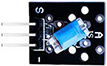
\includegraphics[angle=0, keepaspectratio=true, scale=1, width=200px, height=200px]{images/ball.jpg}
    %\caption{Caption}
\end{figure}
\subsection*{Description}
This module contains a small ball bearing. Operating in a similar fashion to the tilt switch, this module actives when the ball bearing moves to one end of the tube.
\subsection*{Pin mapping}
This pin mapping corresponds to the pins from left to right with the module pins facing towards you.
\begin{table}[H]
    \centering
    \begin{tabular}{|c|c|c|c|c|}
    \hline
    Index &Label &Type &Name &Description\\ \hline
    0 &S &Digital output &D0 &\\ \hline
    1 & &Source voltage &$V+$ &Module source voltage ($5V$)\\ \hline
    2 &- &Ground &GND &\\ \hline
    \end{tabular}
    %\caption{Caption}
    %\label{tab:my_label}
\end{table}
\subsection*{Operation}
When the module is upright the voltage of the digital output pin D0 is low. When the module is in a titled position down the voltage of D0 will be set to high.
\subsection*{Code}
Refer to listing \ref{python_ballswitch}.
%\lstinputlisting[caption=test]{laser.py}